\documentclass[12pt,a4paper,fleqn, onesside]{report}
%
\usepackage[T1]{fontenc}
\usepackage{amsmath, amssymb, amsthm}
\usepackage[danish,english]{babel}

\usepackage[ansinew]{inputenc}
%\usepackage[utf8]{inputenc} %Der skal anvendes utf8
\usepackage{epsfig}
\usepackage{graphicx}
\usepackage[]{mcode}
\usepackage{lmodern}
\usepackage{float}
\usepackage{setspace}
\usepackage{lscape}
\usepackage{hyperref}
\usepackage{cleveref}
\crefname{equation}{}{equations}
\crefname{figure}{figure}{figures}
\usepackage{tabu}
\usepackage{graphicx}
\usepackage{caption}
\usepackage{multirow}
\usepackage{spverbatim}
\onehalfspacing

\usepackage[top=25mm, left=30mm, right=30mm,bottom=25mm,headsep=10mm, footskip=12mm]{geometry}
%
\usepackage{fancyhdr}
\pagestyle{fancyplain}
\lhead[\thepage]{}

\begin{document}

% PAGE DE TITRE
\begin{titlepage}
\begin{center}
\vspace{4cm}
\Huge{\sc 30330 Image Analysis with Microcomputer}\\
\vspace{0.8cm}
\large{\sc Project report\\}
\vspace{1.2cm}
%\Huge {\sc Exam Report}\\
%\vspace{2cm}
\normalsize{by}\\
\vspace{1.2cm}
{\sc
\large Katleen Blanchet s150798  \\ 
Titouan Boulmier s150810\\
}
%\o{}
\vspace{2cm}
\begin{center}

\includegraphics[scale=2.2]{dtulogo2.jpg}
\end{center} 
\vspace{3.1cm}
\normalsize{\today}\\
\vspace{1.37cm}
\includegraphics[scale=0.7]{dtulogo.jpg}\\
\vspace{0.2cm}
\normalsize{Technical University of Denmark \\ Department of Electrical Engineering \\
}
\end{center}
\end{titlepage}
%\newpage
\thispagestyle{empty}
\selectlanguage{english}

\pagebreak
\pagenumbering{Roman}
\setcounter{page}{1}
\setcounter{tocdepth}{4}
\setcounter{secnumdepth}{4} 
\def\chaptername{Part}

% SOMMAIRE
\tableofcontents
\newpage
\pagenumbering{arabic}

% Intro
\section*{Introduction}
\addcontentsline{toc}{part}{Introduction au projet}
The research of habitable planet is one of the major concerns of human beings. Indeed, this discovery, in addition to give hope of locating another species, would bring solutions to overpopulation. According to scientists, the main criterion for life is water. Since the properties of celestial bodies are disparate, a habitable zone was defined, considering that water can only exist at a specific range of temperature. If the temperature of the planet is too low, the water will freeze and conversely, it will evaporate if the temperature is too warm. The habitable zone is not fixed; it moves with the evolution of the sun. Mars is thought to have belonged to the zone once, due to its most hospitable climate after Earth. For a matter of fact, NASA's Mars Reconnaissance Orbiter has recently provided a strong evidence of water currently flowing on the Red Planet. It may then be possible to live on Mars and that is the aim of Mars one project: send a colony over there. The terraforming, which would change characteristics of Mars to make it suitable for humans, is also worth considering before colonization. In order to do so, scientists need to learn more about the features of the planet. Orbiters and rovers are already scanning mars surface and soil. Nevertheless, they lack the depth information, only equipped of Two Dimensional (2D) cameras. Their three dimensional (3D) scans have permitted to acquire it and to print a Martian meteorite on Earth in 2014. This information is useful for a better understanding of the rocks properties but that is not enough. Some missing data have delayed the 3D print. It could be interesting to provide to scientists a real time 3D map of a selected rock. It would be easier to study stones but the map could also help the robot to stabilize. With wind and an uneven ground, the rover is liable to move. The pattern recognition of a rock would be more robust by adding a 3D map. Samples could be collected being sure that the robot has taken the right piece. 

Furthermore, the 3D map could have several other applications. The features of the Martian soil acquired by the orbiting satellites are not exhaustive and lack of accuracy. Thus, applied to the area in front of the robot, the 3D map could detect new obstacles and update in real time the available map to distinguish modifications of the ground. It could also permit spacecrafts to determine a flat area to land in real time by analyzing the surface of the planet from space and during the descent. Moreover, the 3D map has other applications in completely different fields. Indeed, this technical can found, as example, in video games with environment recordings for real time augmented reality gaming, in medicine with skin surface measurement or skin roughness measurement, in cosmetic with wrinkle measurement and also in industry with 3D-automated optical inspection, volume measurement or Classification of grinding materials and tools.

However, the 3D mapping is not much used and is still improving. In this context, designing a system capable of carrying out a 3D map of a Martian rock would be profitable for future research. This is the purpose of this project, undertaken during the Image Analysis with Microcomputer course, under the supervision of Alessandro Massaro. Combining image and scene analysis, programming and robotics seems relevant for learning to work as an engineer.

This report is intended to our fellow students. The first part will bring additional knowledge required to understand the next developments. The design of the system is described in the next section, followed by its verification. To end, future work is addressed.

\chapter{Problem formulation and delimitation}
\section{Problem formulation}
\begin{figure}[H]
  \centering
  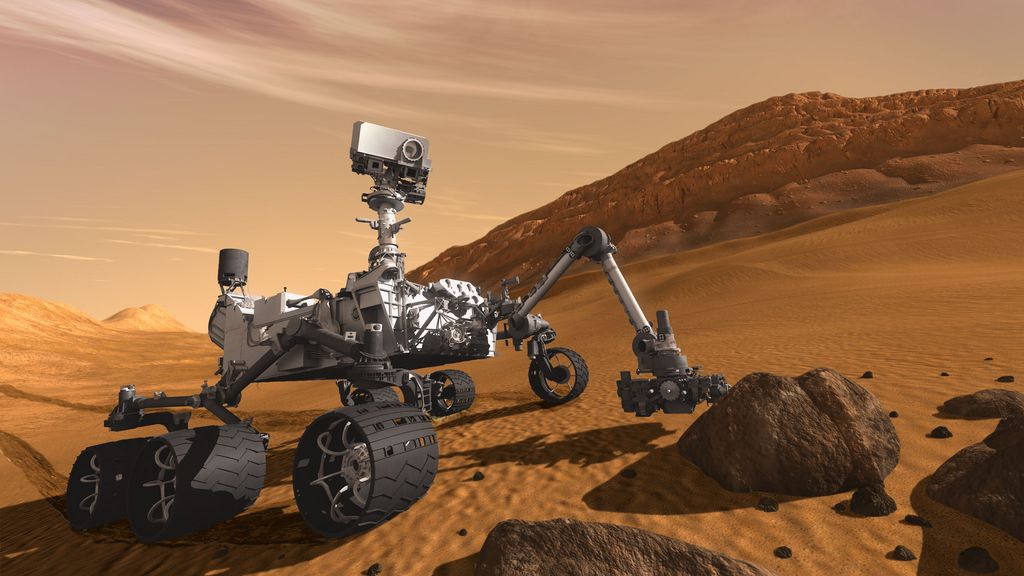
\includegraphics[scale=0.5]{fig/marsRover.jpg}
  \caption{Curiosity Rover with an embedded camera on a arm \cite{nasa}}
  \label{fig:CuriosityRover}
\end{figure}

In this report, we assume that we would like to send a rover on Mars, capable of communicating with Earth. Self-powered by solar panels, it will land at latitude 50� where it could get enough sunlight to recharge its lithium batteries. It is provided with an arm whose hand is replaced with a camera (see figure \ref{fig:CuriosityRover}). The latter will be used by scientists to observe relevant rocks to study. In order to accomplish this mission, once a stone is designed, the camera must be able to keep it in focus, despite the wind, the movement of the robot or any other perturbation. This implies a real time image analysis to be able to rectify the position of the camera. As a robust method is needed to maintain the stone in front of the arm, the correspondence problem is achieved by carrying out a 3D map of the surface. A luminous source should then be added to the rover to be projected on the surface containing the rock and detected by the camera.

This luminous source must be powerful enough to outshine the sunlight during the day, notwithstanding that the energy needed to make it work has to be negligible compared to the amount provided to the rover. Moreover, the characteristics of the camera need to be perfectly adapted to Mars, as once the rover has landed on the red planet, it would be impossible to adjust it. 

Will it be feasible to design such an embedded system, composed of a camera, a luminous source and algorithms, capable of keeping a rock in focus thanks to a 3D map, for an application on Mars soil? 


\section{Problem delimitation}
In order to design the rover's camera which will be used to study rocks and to implement a robust algorithm to carry out a 3D map of the rock's surface, different characteristics of Mars and of the target need to be specified. However, as all of them cannot be taken into account, some simplifications and choices will be assumed.

\paragraph*{Mars delimitation}
~\\
Plenty of missions on Mars have been realized and a great deal of data has already been gathered. Nevertheless, even if some of them will be used to designed our system, others will be simplified or even ignored.
The first simplification concern the atmosphere of Mars. Indeed, even if its composition is now well know, it will be assumed that the dirt on the surface Mars plus the different layers of the atmosphere absorb, or scatter, 10\% of the solar energy. Moreover, the influence on the image acquisition that the dirt between the target and the camera could have will not be taken into account.
The second reduction cover the temperature. Indeed, even if it can reach -143\textdegree C during winter, 27\textdegree C during summer and have around 60\textdegree C variations between daytime and nighttime\cite{wiki:temperature}, we will assume that the CCD sensor works well all the time.

\paragraph*{Target delimitation}
~\\
Regarding the target, that is to say the part of the rock being studied, it is supposed to :
\begin{itemize}
\item be vertical;
\item not exceed 2*2 meters
\item have an area between 0.1 and 1 square meters;
\item have a relief less than  meters.
\end{itemize}

\paragraph*{Camera delimitation}
~\\
Then, regarding the camera which is designed during this study, it is presumed to :
\begin{itemize}
\item be between one and two meters far from the target;
\item be right in front of the target, that is to say that the angle between the normal of the target's surface and the focal axis of the camera is 0\textdegree;
\item be able to capture the image of a target of 2 meters height maximum.
\end{itemize}

The different characteristics of target and the camera are represented figure \ref{fig:schema system}


\begin{figure}[h]
  %\centering
  \centerline{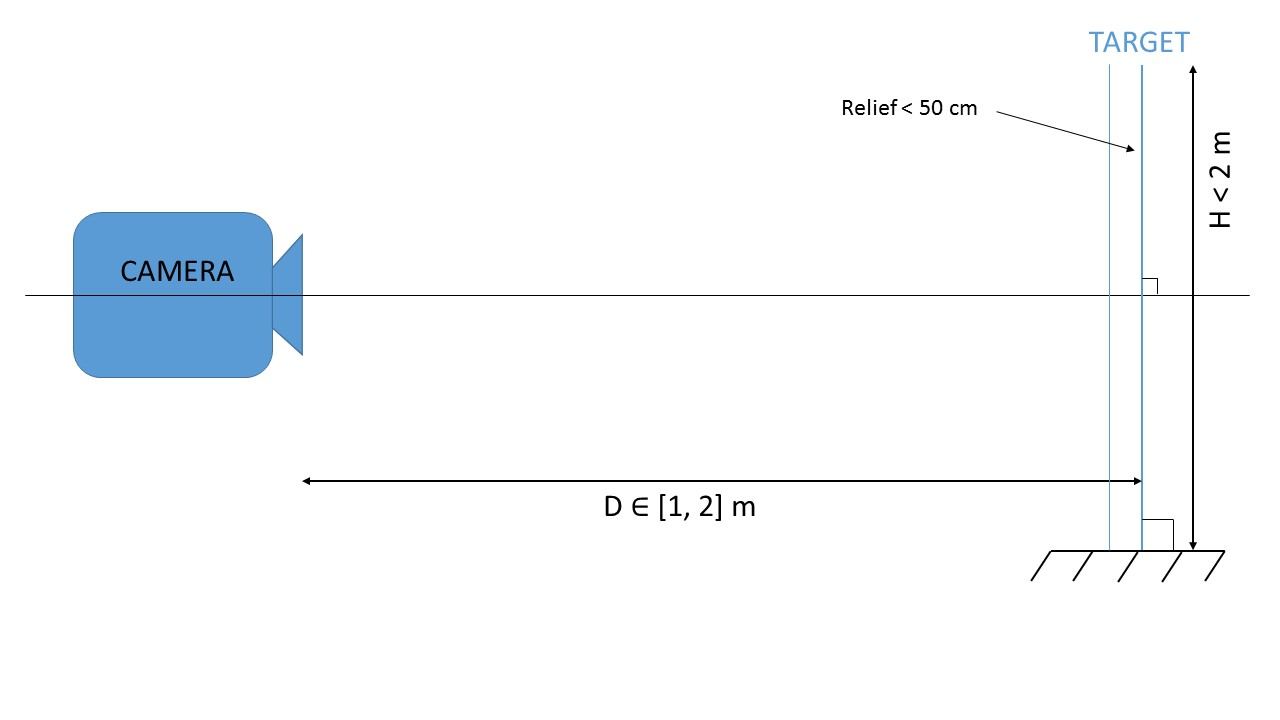
\includegraphics[scale=0.4]{fig/schemaSystem.jpg}}
  \caption{Schema of the scene}
  \label{fig:schema system}
\end{figure}



\chapter{Theory Section}
\section{Scene Analysis}
\subsection{Albedo}
\label{albedo}
Mars surface is covered by sand and volcanic rocks. The first purpose of this project is to allow scientists to examine these rocks through the camera. To achieve it, it is needed to know their characteristics, especially their albedo. As a reminder, the albedo is the fraction of incident light which is reflected from a surface. We can assume that the power reflection of Martian rocks is the same than on Earth. Then, to cover a wild range of rocks, the albedos of a black and of a white stone would be considered. Charcoal, as a dark rock, is a powerful absorber of the sun radiation, with an albedo around 0.05. On the contrary, chalks are poor absorbers and their albedo reach 0.45 according to \cite{albedo}. In the following parts of the report, it will be taken for granted that Martian rocks have an albedo between 5 and 45\%.

\chapter{Development}
\section{Mars Features}
First of all, the irradiance $F$ of the light from the sun falling at the top of the atmosphere of Mars can be calculated as following :
Conservation of energy :
\begin{equation}
\label{eq:conservation of energy}
4\pi R_\odot^2F_\odot=4\pi R^2F
\end{equation}
with 

$R_\odot=6,956.10^8\ m$ : solar radius

$F_\odot=6,45.10^7\ W.m^{-2}$ : energy flow of the surface of the sun

$R \in [2.06644,\ 2.49228].10^{11} \ m$ : distance Mars-Sun (Aphelion and Perihelion)

\begin{equation}
\label{eq:Irradiance Sun range}
F = F_\odot \left(\frac{R_\odot}{R}\right)^2 \in [502, 730]\ W/m^2
\end{equation}

In this report, we will consider that the rover is working on a specific date and we will chose the one when $R$ corresponds to the semi-major axis. In this case $R=2,27936.10^{11}\ km$ and
\begin{equation}
\label{eq:Irradiance Sun}
F = 589\ W/m^2
\end{equation}



Moreover, we can assume that a part of the irradiance is absorbed by the atmosphere. Knowing that the atmosphere of Earth absorbs and scatters to space around 30\% of the incident irradiance of the Sun\cite{yamamoto1962direct}, and knowing  that the atmosphere of Mars is thinner than the one of the Earth, we will postulate that 10\% of the incident irradiance is absorbed. Thus, using \ref{eq:Irradiance Sun} the actual irradiance $F_a$ of the light from the sun falling on the surface of Mars is

\begin{equation}
\label{eq:Actual Irradiance Sun}
F_a = \frac{90}{100}F = \frac{90*589}{100} = 530\ W/m^2
\end{equation}

However, this irradiance is the one of surface exposed perpendicular to the sun's beams. As Mars is a sphere, the projection need to be considered.
Knowing that the weather is better into the northern hemisphere of Mars\cite{wiki:weather} and the fact that a latitude between 30 an 70 degrees is favored for a landing\cite{latitude}, we will assume that the rover has a latitude of 50\textdegree. This latitude corresponds to an angle of 40\textdegree$\ $between the surface of Mars and the sun's beams. Moreover, suppose that the rover stop working when this angle is inferior to 10\textdegree. Thus, the irradiance $F_{50}$ at a latitude of 50\textdegree$\ $is

\begin{equation}
F_{50} = F_asin(angleBeams) \in [92, 341] \ W/m^2
\end{equation}

with $angleBeams = [10, 90-latitude] = [10, 40]$\textdegree.


Then, considering the trajectory of the Sun into the sky of Mars and knowing that the rock target is more or less vertical to the surface of Mars, the angle $\theta$ between the target's normal and the sun's beam is considered to be included in $[10, 50]$\textdegree. In addition, in the optimal case (when all the optimal conditions are provided to have the maximal radiance), the BRDF of the surface of the target is assumed to be 90\% Lambertian and 10\% Glossy while in the worst case the BRDF will be only Lambertian. In this way, the radiance of the target $R_T$ is

\begin{equation}
\label{eq:Radiance Target}
R_T = \left\{
	\begin{array}{ll}
		\frac{F_{50}\alpha}{\pi}\cos \theta & \mbox{ optimal case} \\
		F_{50}\alpha(\frac{9}{10\pi}\cos\theta + \frac{1}{10}) & \mbox{ worst case}
	\end{array}
\right.
\end{equation}

with 
\begin{align*}
	\alpha & \in [0.05, 0.45]\mbox{, the albedo of the target\ref{albedo}} \\
	\theta & \in [10, 50]\mbox{\textdegree, the angle between the target's normal and the sun's beam}
\end{align*}
Thus, 
\begin{equation}
R_T \in [92, 340] \ W/m^2
\end{equation}







\bibliography{bibliographie}
\bibliographystyle{plain}

\end{document}
